

\subsection{Камеры}

\begin{frame}{Видеоаналитика (1)}
    \begin{orange-box}{Полуавтоматическое наблюдение}
        \begin{itemize}
            \item[$\Leftarrow$] Пульт оператора:
            \begin{itemize}
                \item много камер;
                \begin{itemize}
                    \item система наблюдения банка 
                    $\approx 200$ камер.
                \end{itemize}
                \item просматривает человек;
                \item не всегда понятно на какой из камер <<тревога>>;
            \end{itemize}
            \item[${\color{red}\Rightarrow}$] Оповещение — на что обратить внимание оператору.
        \end{itemize}
    \end{orange-box}
    \vspace{1.5em}
    \begin{blue-box}{Быстрая навигация по видео}
        \begin{itemize}
            \item[$\Leftarrow$] Много видео c камер:
            \begin{itemize}
                \item просматривают только когда <<что-то случается>>;
                \item невозможно среагировать до того, как случилось.
            \end{itemize}
            \item[${\color{red}\Rightarrow}$] Метки когда 
            происходило что-то необычное.
        \end{itemize}
    \end{blue-box}
\end{frame}

\begin{frame}{Видеоаналитика (2)}
    \begin{center}
        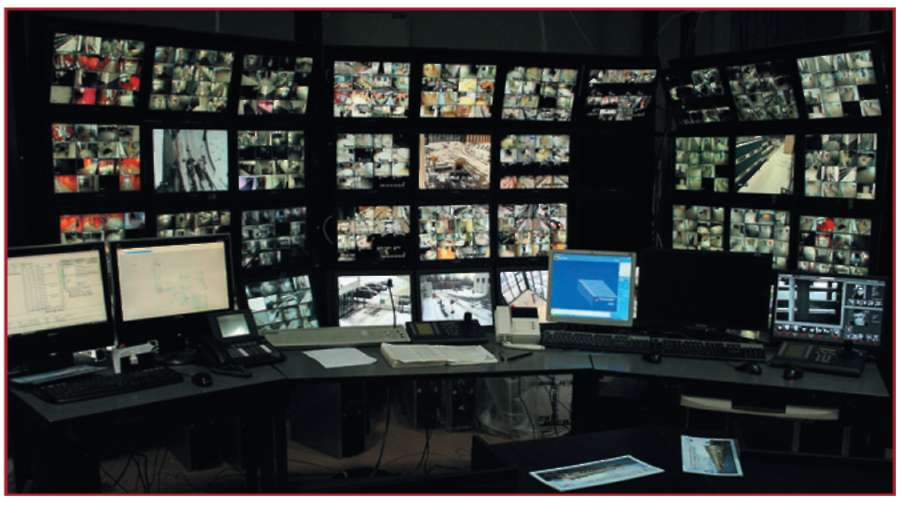
\includegraphics[width=\textwidth]{img/video/cctv.jpg}
    \end{center}
\end{frame}

\begin{frame}{Видеоаналитика (3)}
 
    \begin{gray-box}{Поиск шаблонов действий}
        \begin{itemize}
            \item похожие, но разные:
            \begin{itemize}
                \item «человек подходит к двери и открывает ее»;
                \item «человек подходит к двери и уходит».
            \end{itemize}
        \end{itemize}
    \end{gray-box}
    \vspace{2em}
    \begin{orange-box}{Проблемы}
        \begin{itemize}
            \item разные варианты реализации шаблона;
            \item «шум»:
            \begin{itemize}
                \item прохожие;
                \item падающие листья;
                \item ...;
            \end{itemize}
            \item детекторы движения (часто) бесполезны.
        \end{itemize}
    \end{orange-box}
\end{frame}

\subsection{БПЛА}

\begin{frame}{Поиск шаблонов: навигация БПЛА}
    \begin{center}
        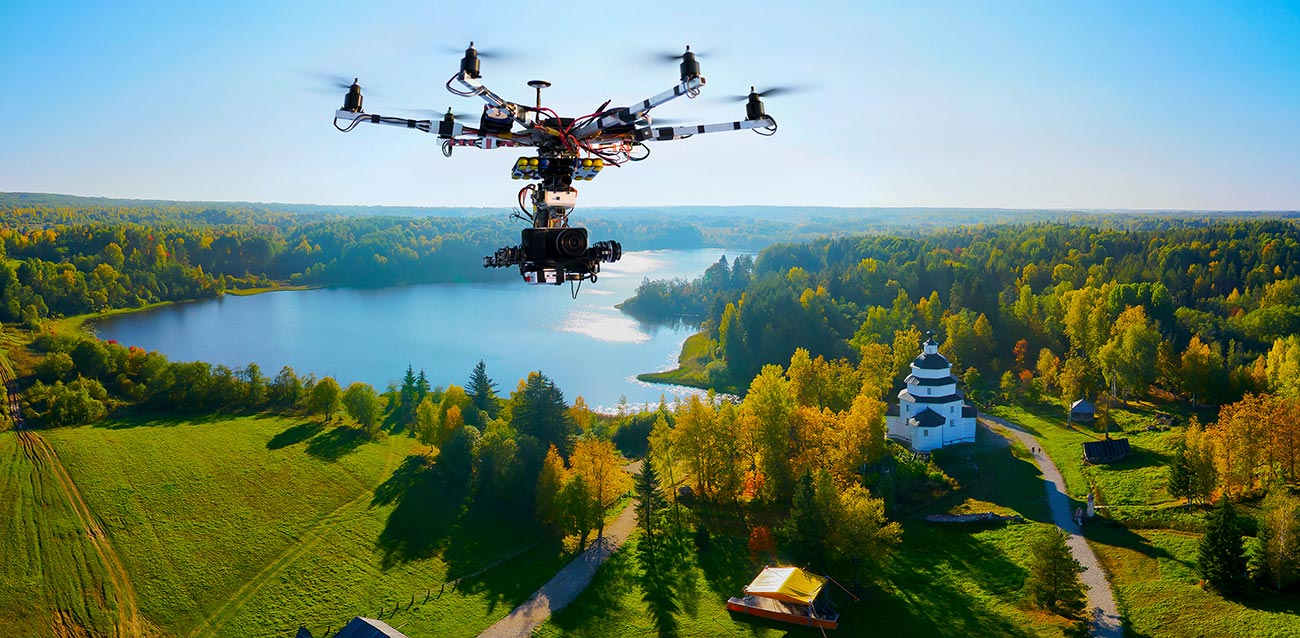
\includegraphics[width=\textwidth]{img/video/drone-3.jpg}
    \end{center}
    \begin{gray-box}{Пример}
        \begin{itemize}
            \item «пролетели над озером, потом над полем».
        \end{itemize}
    \end{gray-box}
\end{frame}

\begin{frame}{Навигация БПЛА}
    \begin{blue-box}{Кто использует:}
        фотографы, путешественники, геодезисты, геологи.
        \vspace{0.5em}
        \begin{center}
            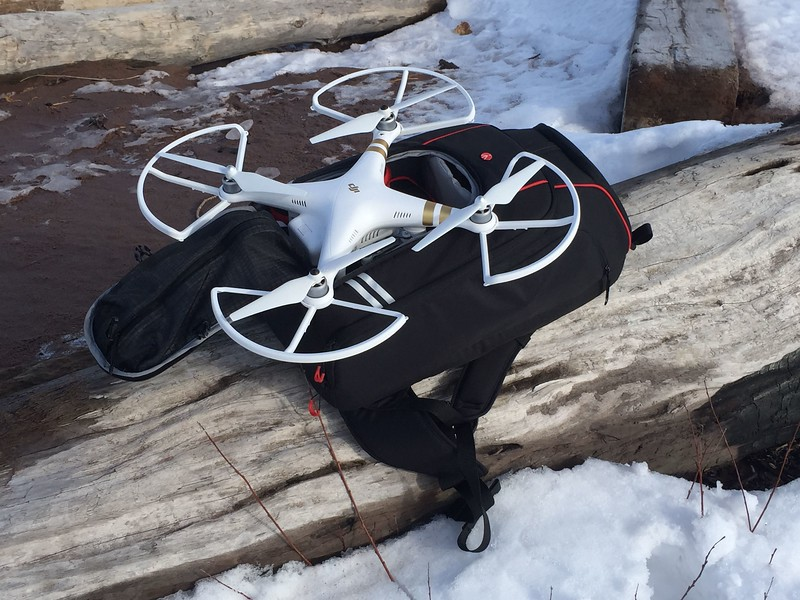
\includegraphics[width=7cm]{img/video/drone-2.jpg}
        \end{center}
        \vspace{0.5em}
    \end{blue-box}
\end{frame}

